\documentclass[tikz,border=10pt]{standalone}
\usetikzlibrary{arrows.meta, positioning, calc}
\usepackage{amssymb}

\begin{document}
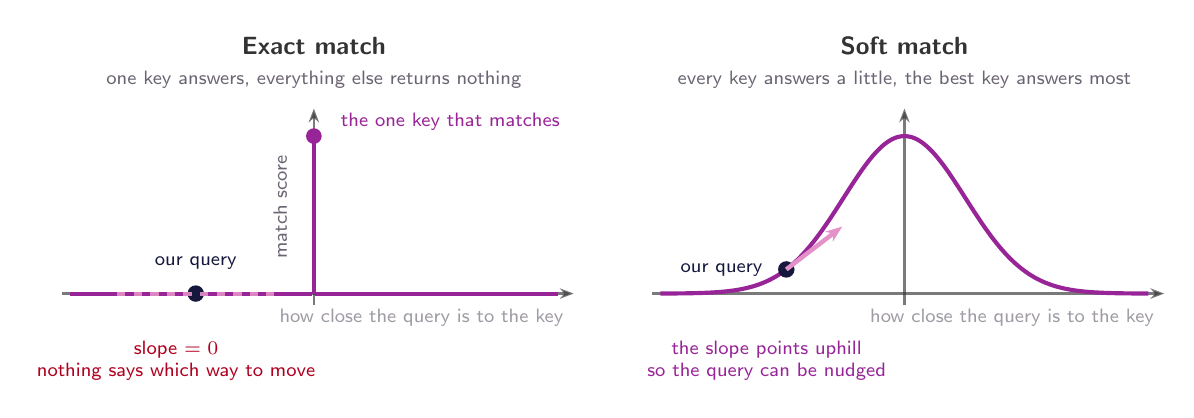
\begin{tikzpicture}[
    every node/.style={font=\sffamily},
]

% ---------------------------------------------------------------- colours
\definecolor{c1}{HTML}{15173D}   % the query, and the axes
\definecolor{c2}{HTML}{982598}   % the match score curve
\definecolor{c3}{HTML}{E491C9}   % the slope we can follow
\definecolor{c4}{HTML}{F1E9E9}
\definecolor{axiscolor}{HTML}{333333}
\definecolor{labelcolor}{HTML}{6B6472}
\definecolor{deadred}{HTML}{B00020}

% ---------------------------------------------------------------- styles
\tikzset{
    axis/.style={-{Stealth[length=5pt]}, line width=0.8pt, axiscolor,
                 opacity=0.65},
    curve/.style={c2, line width=1.5pt},
    qdot/.style={circle, fill=c1, inner sep=2.1pt},
}

% ================================================================
% Each panel is drawn in data coordinates, x in [-3, 3], y in [0, 2.2],
% and shifted into place. Panel A is centred at x = 3.5, panel B at 11.
% ================================================================

% ----------------------------------------------------------------------
% PANEL A: exact match
% ----------------------------------------------------------------------
\begin{scope}[shift={(3.5, 0)}]

    \node[font=\sffamily\small\bfseries, text=axiscolor] at (0, 3.15)
        {Exact match};
    \node[font=\sffamily\scriptsize, text=labelcolor] at (0, 2.72)
        {one key answers, everything else returns nothing};

    \draw[axis] (-3.2, 0) -- (3.3, 0)
        node[anchor=north east, font=\sffamily\scriptsize, text=labelcolor,
             yshift=-2pt] {how close the query is to the key};
    \draw[axis] (0, -0.15) -- (0, 2.35);
    \node[font=\sffamily\scriptsize, text=labelcolor, rotate=90, anchor=south]
        at (-0.22, 1.1) {match score};

    % the score: zero everywhere, one single spike at the key
    \draw[curve] (-3.1, 0) -- (-0.02, 0);
    \draw[curve] (0.02, 0) -- (3.1, 0);
    \draw[curve] (0, 0) -- (0, 2.0);
    \node[circle, fill=c2, inner sep=2pt] at (0, 2.0) {};
    \node[font=\sffamily\scriptsize, text=c2, anchor=west] at (0.22, 2.18)
        {the one key that matches};

    % our query sits somewhere off the key
    \node[qdot] (qa) at (-1.5, 0) {};
    \node[font=\sffamily\scriptsize, text=c1, anchor=south] at (-1.5, 0.18)
        {our query};

    % the slope here is flat, in both directions
    \draw[c3, line width=1.4pt, dashed, opacity=0.9]
        (-2.5, 0) -- (-0.5, 0);
    \node[font=\sffamily\scriptsize, text=deadred, align=center]
        at (-1.75, -0.85) {slope $=0$\\nothing says which way to move};

\end{scope}

% ----------------------------------------------------------------------
% PANEL B: soft match
% ----------------------------------------------------------------------
\begin{scope}[shift={(11, 0)}]

    \node[font=\sffamily\small\bfseries, text=axiscolor] at (0, 3.15)
        {Soft match};
    \node[font=\sffamily\scriptsize, text=labelcolor] at (0, 2.72)
        {every key answers a little, the best key answers most};

    \draw[axis] (-3.2, 0) -- (3.3, 0)
        node[anchor=north east, font=\sffamily\scriptsize, text=labelcolor,
             yshift=-2pt] {how close the query is to the key};
    \draw[axis] (0, -0.15) -- (0, 2.35);
    % no "match score" label on this panel: the bump runs straight through
    % where it would sit, and both panels share the same axes anyway

    % score = 2 exp(-x^2 / 1.2)
    \draw[curve, domain=-3.1:3.1, samples=120, smooth]
        plot (\x, {2*exp(-(\x)*(\x)/1.2)});

    % our query, at the same place as in panel A
    % at x = -1.5:  y  = 2 exp(-2.25/1.2) = 0.3067
    %               y' = y * (-2x/1.2)   = 0.767  (uphill, towards the key)
    \node[qdot] (qb) at (-1.5, 0.3067) {};
    \node[font=\sffamily\scriptsize, text=c1, anchor=east] at (-1.68, 0.30)
        {our query};

    \draw[c3, line width=1.6pt, -{Stealth[length=6pt]}]
        (-1.5, 0.3067) -- (-0.79, 0.851);
    \node[font=\sffamily\scriptsize, text=c2, align=center]
        at (-1.75, -0.85) {the slope points uphill\\so the query can be nudged};

\end{scope}

\end{tikzpicture}
\end{document}
